\section{Attori}
\label{sec:attori}
\subsection{\textit{Sync}}
\paragraph{} 
\textit{Sync} rappresenta il sincronizzatore remoto, un web service esterno che si interfaccia con una serie di servizi tra cui \textit{Esse3}, ossia il portale dello studente che offre le funzionalità da replicare nell’applicazione, \textit{Aule Unimol} ed altri servizi esterni. È un’entità esterna al sistema che si vuole realizzare, pertanto  è classificata come attore.
\begin{center}
	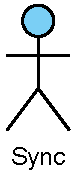
\includegraphics[width=0.6in]{imgs/attori/Attore-Sync.pdf}
\end{center}

\subsection{\textit{Docente}}
\paragraph{} 
\textit{Docente} è un professore dell’\textit{Università degli Studi del Molise} avente le credenziali di accesso al portale \textit{Esse3}. Il \textit{Docente} utilizzerà la nuova funzionalità per comunicare in modo rapido e semplice e anche in via ufficiosa con tutti gli studenti che frequentano un proprio corso. Egli potrà amministrare le chat secondo le sue preferenze, in particolare potrà creare o rimuovere dei canali e aggiungere o rimuovere i membri.
\begin{figure}[h]
	\centering
	
\includegraphics[width=0.6in]{imgs/attori/Docente.png}
	\caption{Attore: Docente chat}
	\label{fig:Attore: Docente chat}
\end{figure}

\subsection{Studente}
\paragraph{} 
Studente regolarmente iscritto all’\textit{Università degli Studi Del Molise}, munito delle credenziali per accedere al portale dello studente \textit{Esse3}, il servizio esterno sul quale si basa l’applicazione. Lo studente utilizza l’applicazione per usufruire in maniera agevole dei servizi offerti dai portali dell’\textit{Università degli Studi del Molise} e monitorare la propria carriera universitaria. Di seguito è mostrata l'icona dello studente standard.
\begin{center}
	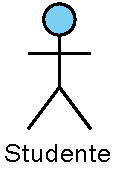
\includegraphics[width=0.8in]{imgs/attori/Attore-Studente.pdf}
\end{center}
Per quanto riguarda la nuova funzionalità di messaggistica, lo \textit{Studente} utilizzerà tale funzione per facilitare la comunicazione ufficiale con i docenti relativi ai corsi della Coorte di appartenenza. Potrà comunicare, inoltre, con gli altri studenti appartenenti al suo stesso anno di corso. Di seguito è mostrato lo studente della chat.
\begin{figure}[h]
	\centering
	
\includegraphics[width=0.6in]{imgs/attori/Studente.png}
	\caption{Attore: Studente chat}
	\label{fig:Attore: Studente chat}
\end{figure}

\subsection{Amministratore}
\paragraph{} 
E' un Amministratore dell’\emph{Università degli Studi del Molise}, al quale sono assegnate le credenziali per poter effettuare l’accesso al pannello amministrazione.\emph{L’Amministratore} avrà il compito di gestire, mediante tale pannello, le \emph{chat} degli studenti e le \emph{chat} dei corsi dove potrà coordinare i relativi canali e gli utenti in essi presenti.
Avrà anche la possibilità di inviare notifiche personalizzate e di gestire la segnalazione dei messaggi inopportuni all’interno delle \emph{chat}.

\begin{figure}[h]
	\centering
	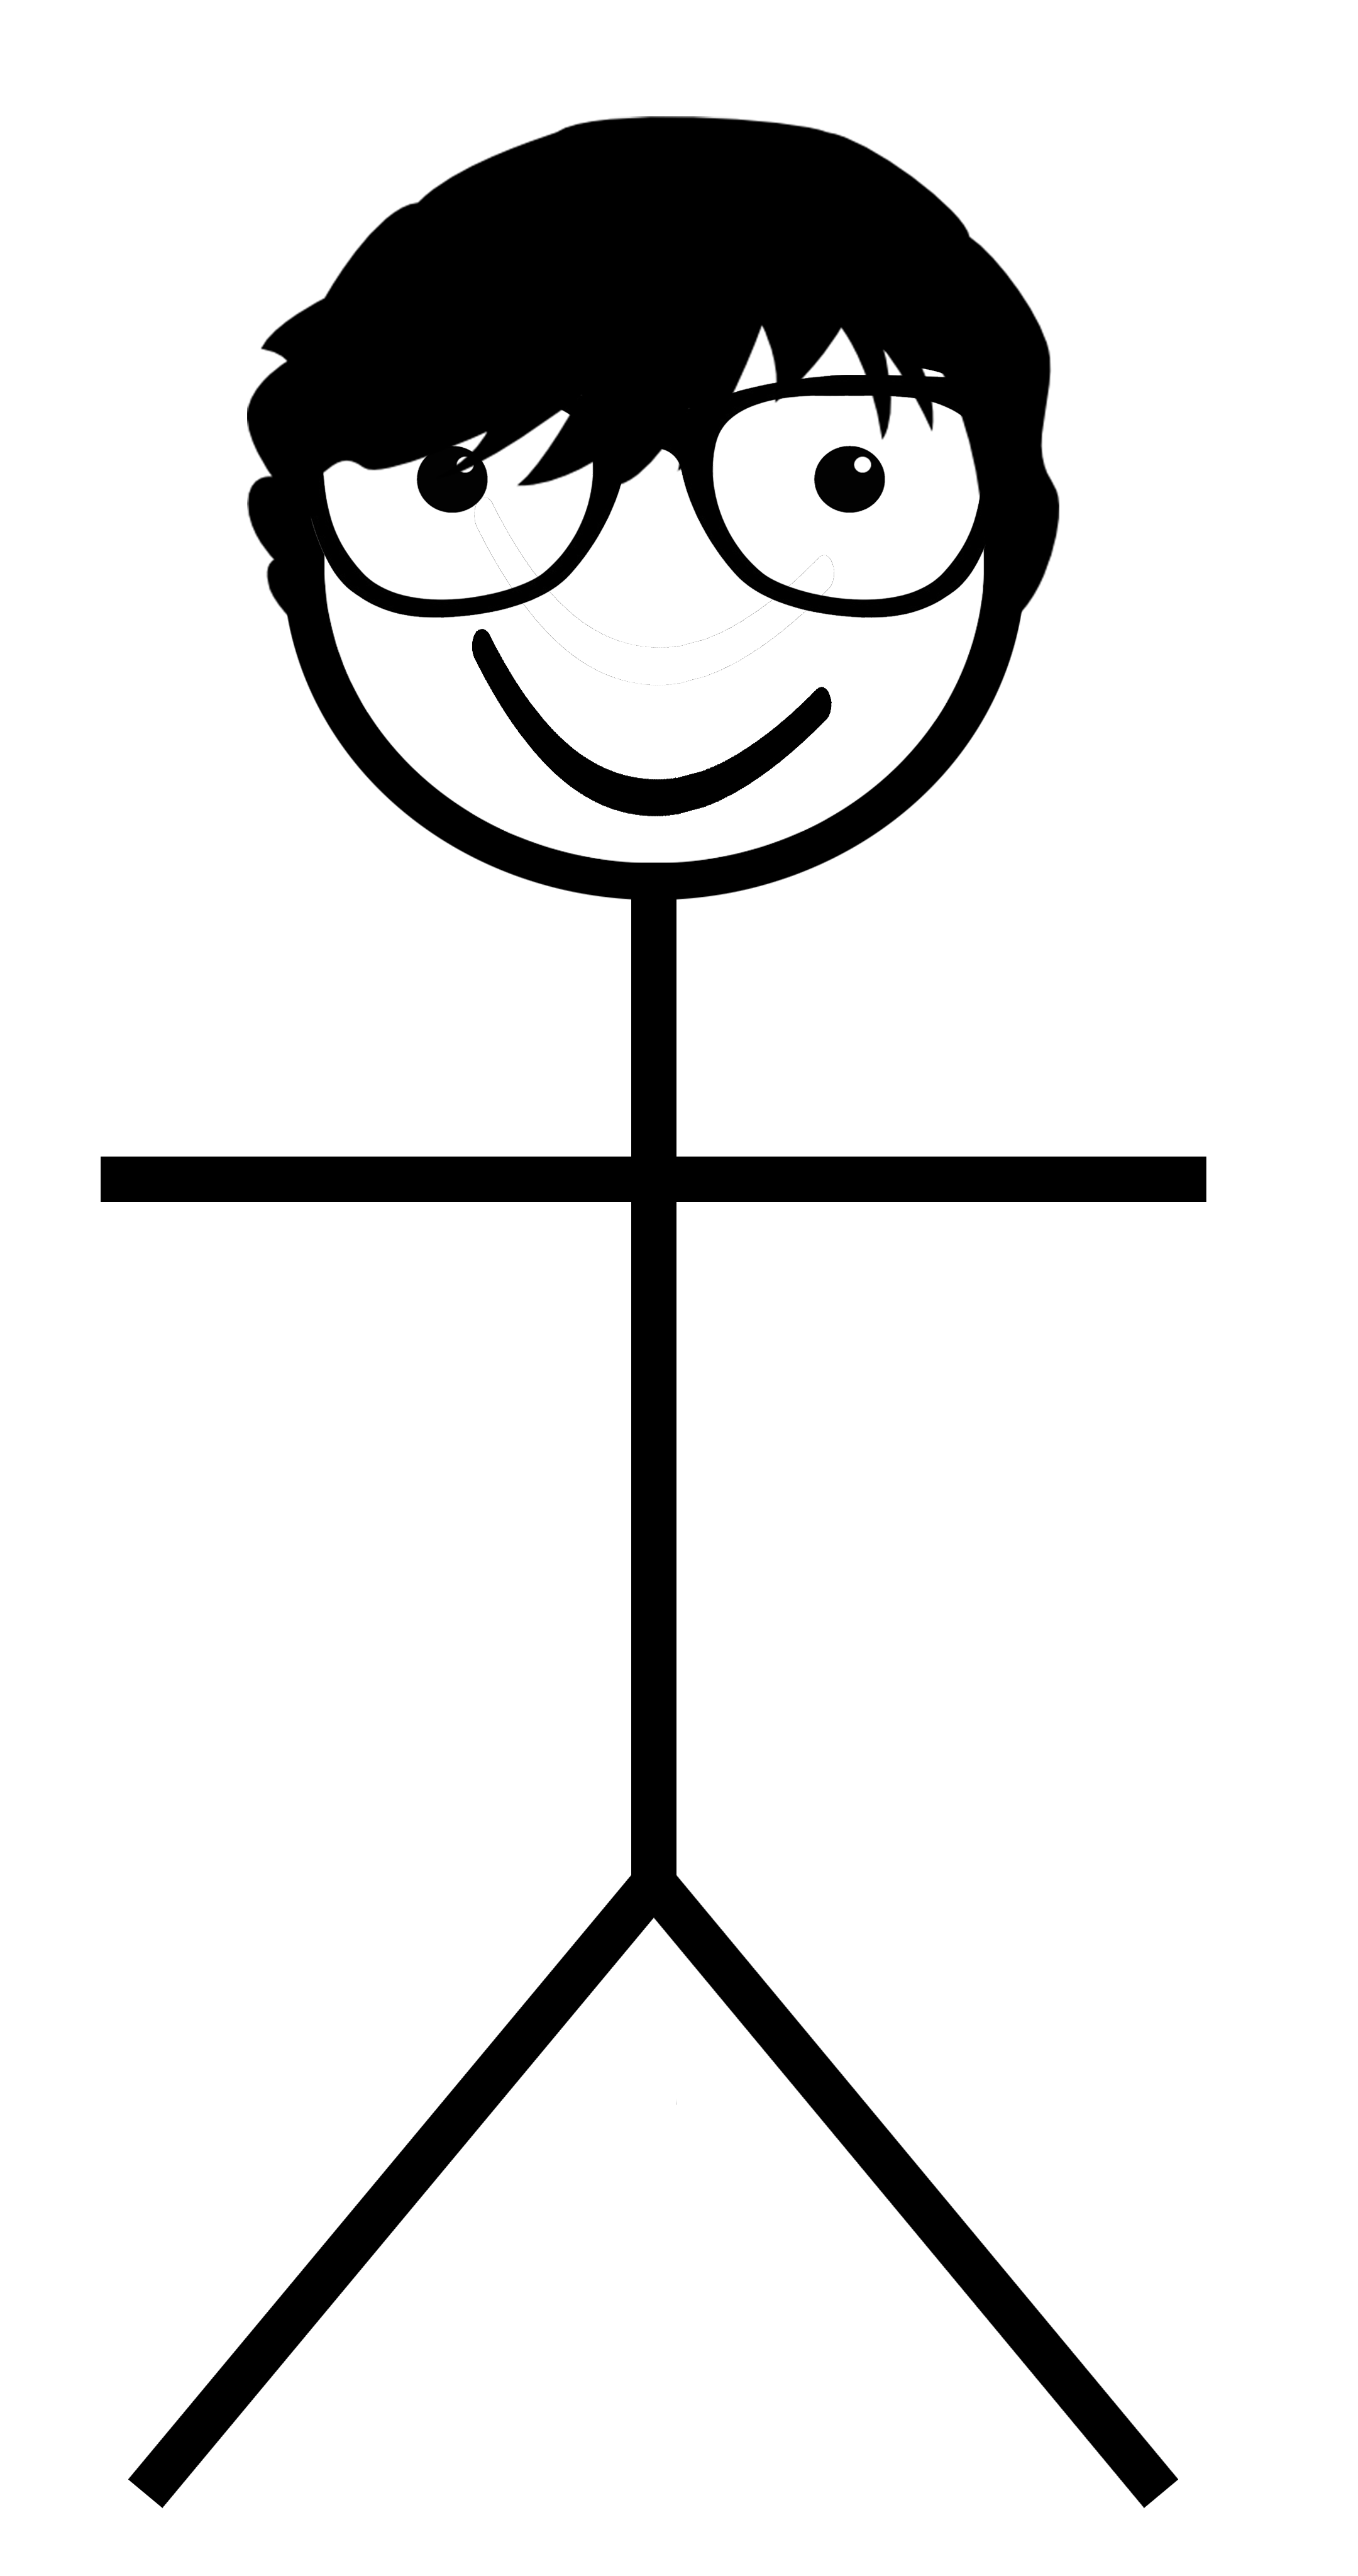
\includegraphics[width=0.6in]{imgs/attori/admin.png}
	\caption{Attore: Amministratore}
	\label{fig:Attore: Amministratore} 
\end{figure}

\clearpage